\documentclass[11pt,a4paper]{article}

% ══════════════════════════════════════════════════════════════════════════════
%  PACKAGES
% ══════════════════════════════════════════════════════════════════════════════
\usepackage[T1]{fontenc}
\usepackage[utf8]{inputenc}
\usepackage{amsmath,amssymb,amsfonts,amsthm}
\usepackage{graphicx}
\graphicspath{{figures/}}
\usepackage{bm}
\usepackage{siunitx}
\usepackage{geometry}
\usepackage[colorlinks=true,linkcolor=black,citecolor=blue,urlcolor=blue]{hyperref}
\usepackage[noabbrev,nameinlink]{cleveref}
\usepackage{xcolor}
\usepackage{booktabs}
\usepackage{enumitem}
\usepackage{float}
\usepackage{natbib}
\usepackage{tcolorbox}

\geometry{margin=1in}

% Custom theorem environments
\newtheorem{assumption}{Assumption}
\theoremstyle{definition}
\newtheorem{definition}{Definition}

% Colored boxes for key results
\tcbuselibrary{theorems}
\newtcolorbox{keyresult}{colback=blue!5!white,colframe=blue!75!black,title=Key Result}
\newtcolorbox{criterion}{colback=green!5!white,colframe=green!50!black,title=Priming Criterion}

% ══════════════════════════════════════════════════════════════════════════════
%  TITLE
% ══════════════════════════════════════════════════════════════════════════════
\title{\textbf{Theory and Experiments on Self-Starting Siphons}\\[0.5em]
       \large A One-Dimensional Slug-Flow Model with Layered Analysis\\[0.75em]
       \rule{0.6\textwidth}{0.4pt}\\[0.5em]
       \normalsize IYPT 2026 --- Problem \#1}
\author{Stelios Raptopoulos}
\date{December 2024}

\begin{document}
\maketitle

% ══════════════════════════════════════════════════════════════════════════════
%  ABSTRACT
% ══════════════════════════════════════════════════════════════════════════════
\begin{abstract}
A self-starting siphon primes spontaneously when partially immersed, requiring no external suction. We develop a one-dimensional slug-flow model through systematic layered analysis, progressively incorporating physical effects to understand how parameters control priming success and filling time.

Starting from the Navier-Stokes equations, we derive the governing ordinary differential equation through explicit simplifications: incompressibility, axisymmetry, quasi-steady velocity profiles, and rigid-slug dynamics. The frictionless limit yields the energy integral $I(L)$, computable analytically for piecewise-linear geometries. Container drawdown introduces the area ratio $A/A_0$, while friction adds pipe roughness $\varepsilon/D$ and bend losses $K$. Comparing these three analytical integrals reveals the energy cost of each effect.

Comparison with video-tracked measurements shows that the full numerical model, with its minor-loss coefficient fitted to those measurements, reproduces the essential dynamics, while the analytical bounds provide physical insight unavailable from simulation alone. Validity limits---cavitation, capillarity, entrance effects, and secondary flows---are quantified through dimensionless parameters (Bond, capillary, Dean, and Womersley numbers) and visualized in regime diagrams.
\end{abstract}

\tableofcontents
\newpage

% ══════════════════════════════════════════════════════════════════════════════
%  SECTION 1: INTRODUCTION
% ══════════════════════════════════════════════════════════════════════════════
\section{Introduction}
\label{sec:intro}

The International Young Physicists' Tournament (IYPT) 2026 Problem~\#1 poses the following challenge:
\begin{quote}
\emph{``A self-starting siphon can be made using a piece of rigid tubing bent into a specific shape. When the siphon is partially immersed in water, it begins siphoning water without the need for initial suction. Investigate how the relevant parameters, such as the geometry, affect the siphoning process.''}
\end{quote}

\subsection{Physical Background}

The siphon has fascinated scientists since antiquity. While its operation was long attributed to atmospheric pressure, modern understanding recognizes that gravity provides the fundamental driving mechanism \citep{boatwright2015siphon}. In a standard siphon, liquid flows from a higher reservoir to a lower one through an inverted U-tube, even though part of the path rises above the source reservoir. The key insight is that the liquid column acts as a continuous chain: water descending the outlet leg ``pulls'' water up the inlet leg through cohesive forces.

A \emph{self-starting} siphon eliminates the need for manual priming. Through clever geometry---typically involving an internal drop and rise sequence---the siphon uses momentum gained during an initial descent to carry water over a crest above the waterline. Once primed, ordinary siphon action drains the container.

\subsection{Previous Work}

The physics of siphons has been revisited periodically in the literature. \citet{mcdonald2024siphon} provides a detailed force analysis, while \citet{potter2012siphon} explores the role of molecular cohesion. The Bernoulli equation approach is standard in fluid mechanics textbooks \citep{white2011fluid,fox2011introduction}, though the transient filling dynamics of self-starting siphons have received less attention.

\subsection{Approach and Contributions}

This paper develops a theoretical framework through layered analysis:
\begin{enumerate}[nosep,leftmargin=2em]
  \item \textbf{Navier-Stokes derivation} (\cref{sec:navier-stokes}): We begin from first principles, making each simplification explicit and showing how the governing equation transforms at each step.
  \item \textbf{Frictionless model} (\cref{sec:frictionless}): With friction neglected, geometry alone determines the outcome through the energy integral $I(L)$.
  \item \textbf{Drawdown effects} (\cref{sec:drawdown}): The area ratio $A/A_0$ controls how the container level falls.
  \item \textbf{Friction effects} (\cref{sec:friction}): Pipe roughness and bend losses are incorporated using the Darcy-Weisbach equation \citep{brown2002history}.
  \item \textbf{Model comparison} (\cref{sec:comparison}): Three analytical integrals visualize the hierarchy of effects.
  \item \textbf{Numerical dynamics} (\cref{sec:dynamics}): Velocity-dependent friction requires numerical integration.
  \item \textbf{Comparison with experiment} (\cref{sec:experiments}): Video tracking provides velocity measurements.
  \item \textbf{Validity limits} (\cref{sec:validity}): Dimensionless parameters quantify when assumptions fail.
\end{enumerate}

% ══════════════════════════════════════════════════════════════════════════════
%  SECTION 2: PHYSICAL SETUP
% ══════════════════════════════════════════════════════════════════════════════
\section{Physical Setup}
\label{sec:setup}

\subsection{Coordinate System and Geometry}

We work in a vertical plane with horizontal coordinate $x$ (rightward positive) and vertical coordinate $h$ (upward positive), with datum $h = 0$ at the container base.

The pipe centreline connects five nodes by straight segments:
\begin{equation}
  A = (x_0, h_0), \quad B = (x_1, h_1), \quad C = (x_2, h_2), \quad D = (x_3, h_3), \quad E = (x_4, h_4).
  \label{eq:nodes}
\end{equation}

Each node has a physical role:
\begin{center}
\renewcommand{\arraystretch}{1.2}
\begin{tabular}{cl}
\toprule
Node & Physical Role \\
\midrule
$A$ & Inlet, near container bottom \\
$B$ & First crest, below initial water level \\
$C$ & Low point of internal drop (velocity peaks here) \\
$D$ & Main crest, \emph{above} the initial water level \\
$E$ & Outlet, at or below container bottom \\
\bottomrule
\end{tabular}
\end{center}

The defining constraint for self-starting is $h_1 < h_c^{(0)} < h_3$: the first crest lies below the waterline, the main crest above it.

\subsection{Arclength Parameterization}

The arclength $L$ measures distance along the pipe from the inlet. On segment $i$ (for $L \in [S_{i-1}, S_i]$), the centreline elevation follows:
\begin{equation}
  h(L) = c_i + s_i L,
  \label{eq:hL-piecewise}
\end{equation}
where $s_i = \sin\theta_i = (h_i - h_{i-1})/L_i$ is the slope and $c_i = h_{i-1} - s_i S_{i-1}$ ensures continuity.

\subsection{Critical Points}

Point $W$ marks where the descending front crosses the waterline for the last time on segment $D \to E$:
\begin{equation}
  h(S_W) = h_c^{(0)} \quad \Rightarrow \quad S_W = \frac{h_c^{(0)} - c_4}{s_4}.
  \label{eq:SW-def}
\end{equation}

Point $W'$ marks the ascending crossing on segment $C \to D$. Between $W'$ and $W$, the front is above the waterline and experiences negative driving force.

\subsection{Experimental Parameters}

\Cref{tab:parameters} lists all parameters for the worked example, derived from our experimental setup.

\begin{table}[H]
\centering
\caption{Complete parameter set for the experimental siphon.}
\label{tab:parameters}
\renewcommand{\arraystretch}{1.15}
\small
\begin{tabular}{llll}
\toprule
\multicolumn{4}{l}{\textbf{Geometry}} \\
\midrule
Node & $x$ (cm) & $h$ (cm) & Role \\
\midrule
$A$ & 0.0 & 1.0 & Inlet \\
$B$ & 7.5 & 11.0 & First crest \\
$C$ & 13.5 & 5.0 & Low point \\
$D$ & 21.4 & 13.0 & Main crest \\
$E$ & 30.3 & $-1.7$ & Outlet \\
\midrule
\multicolumn{4}{l}{Initial water level: $h_c^{(0)} = 12.5$\,cm \quad Total length: $L_{\max} = 49.41$\,cm} \\
\midrule
\multicolumn{4}{l}{\textbf{Pipe Properties}} \\
\midrule
Inner diameter & $D = 5$\,mm & Cross-section & $A = 0.196\,\text{cm}^2$ \\
Relative roughness & $\varepsilon/D \approx 3.5\times 10^{-4}$ & Minor losses & $\sum K \approx 14.4$ (fitted) \\
\midrule
\multicolumn{4}{l}{\textbf{System Parameters}} \\
\midrule
Container area & $A_0 = 340\,\text{cm}^2$ & Area ratio & $A/A_0 = 5.77\times 10^{-4}$ \\
Water density & $\rho = 998\,\text{kg/m}^3$ & Viscosity & $\nu = 1.0 \times 10^{-6}\,\text{m}^2/\text{s}$ \\
Surface tension & $\gamma = 0.073\,\text{N/m}$ & Gravity & $g = 9.81\,\text{m/s}^2$ \\
\bottomrule
\end{tabular}
\end{table}

% --- FIGURE 1: Geometry ---
\begin{figure}[H]
  \centering
  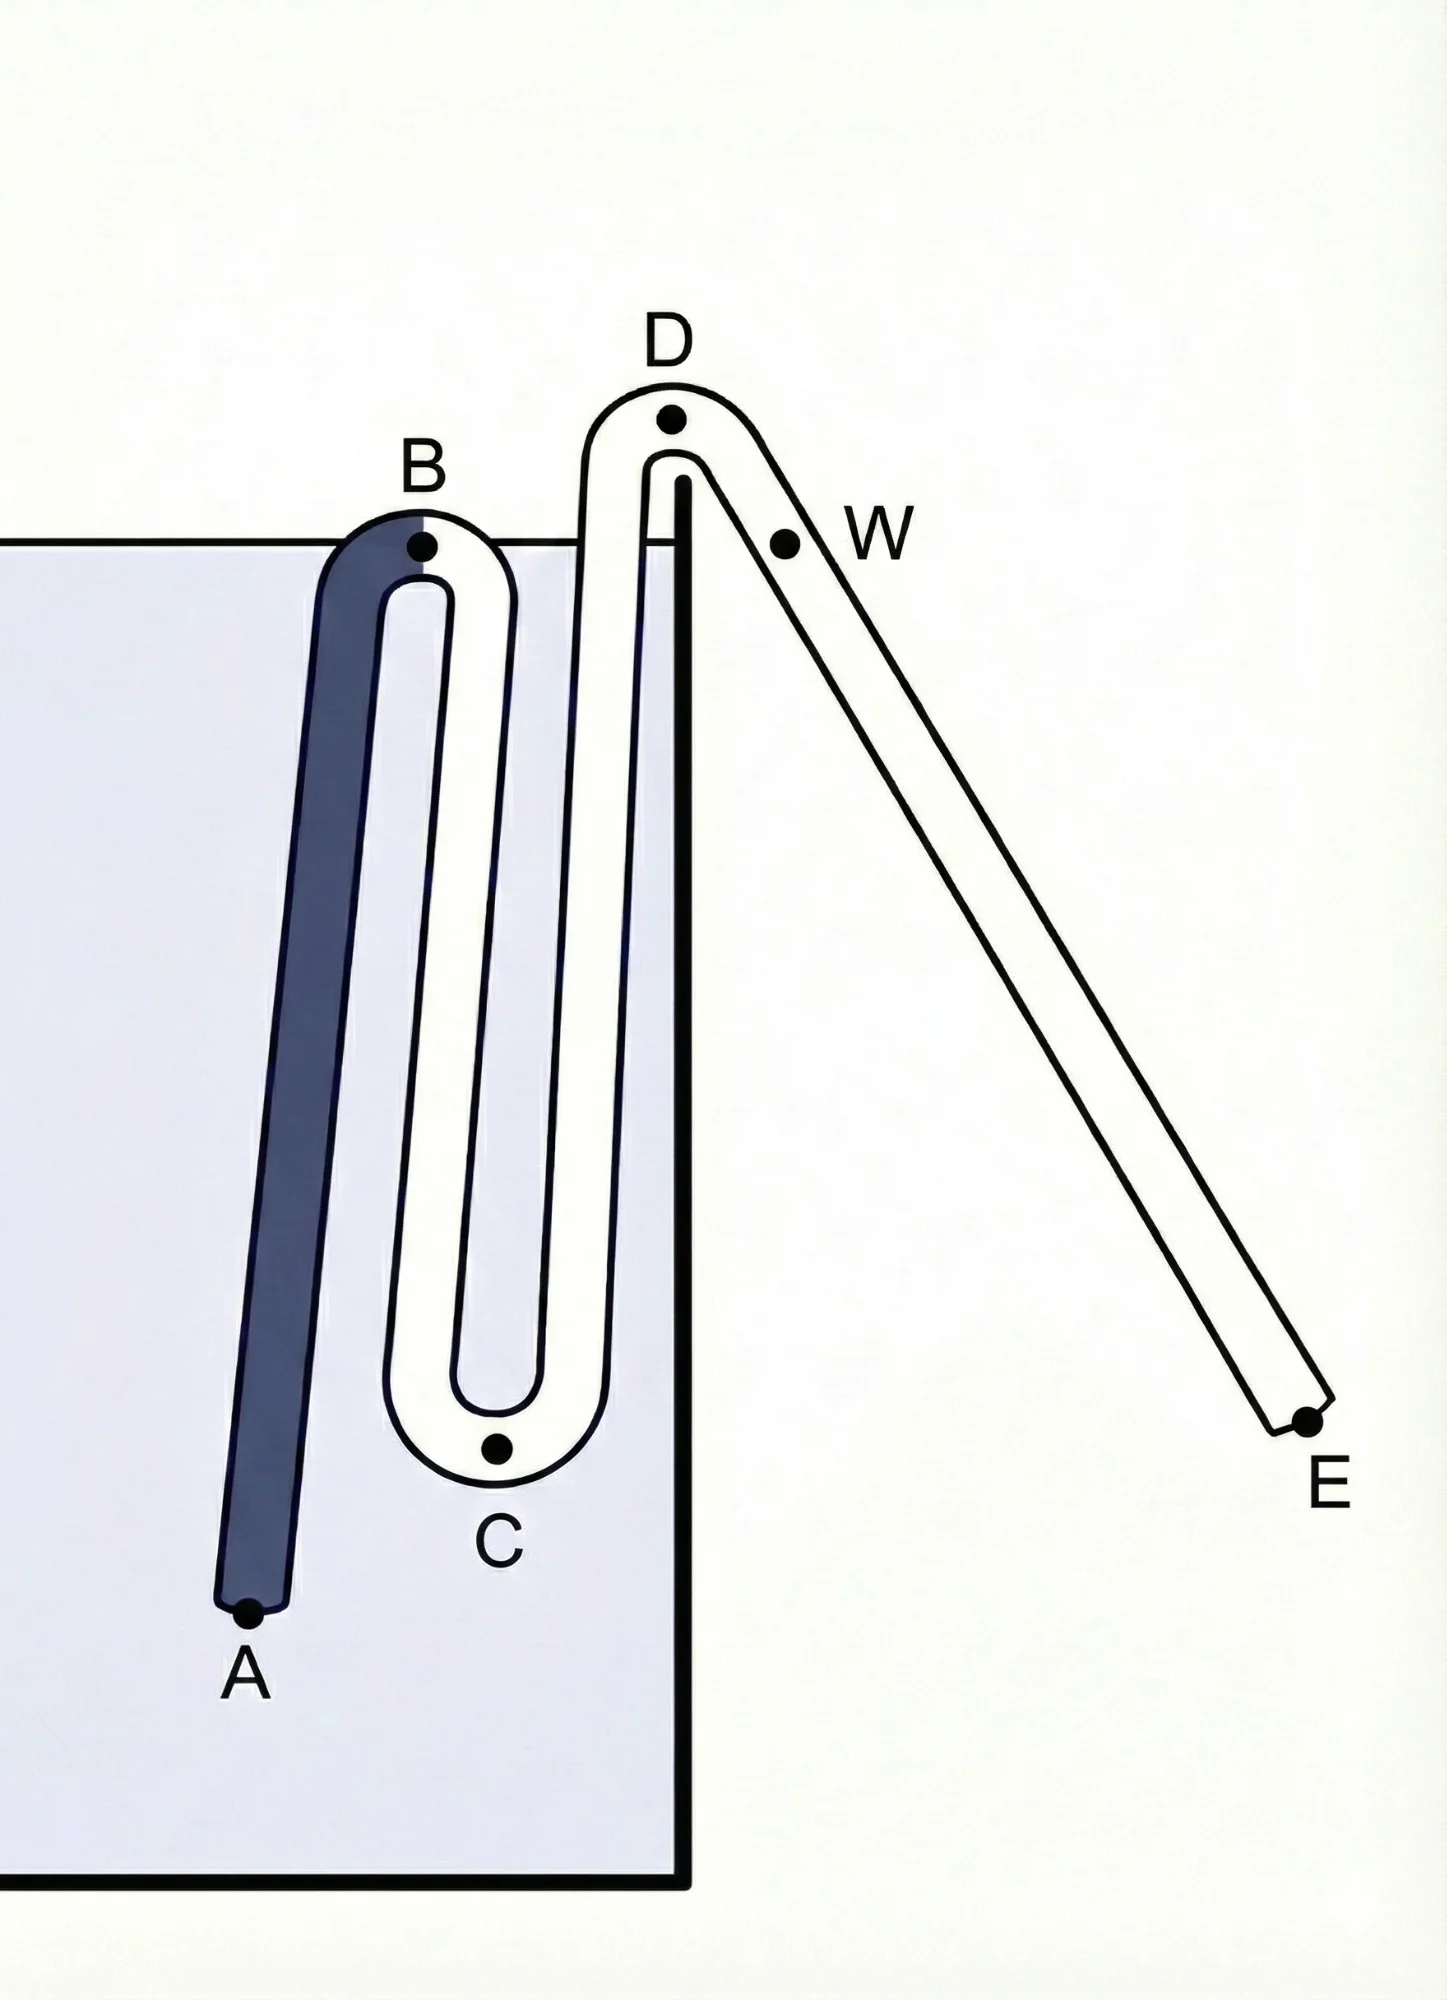
\includegraphics[width=0.55\textwidth]{siphon_schematic.png}
  \caption{Schematic of the self-starting siphon. The water level $h_c^{(0)}$ lies between crests $B$ and $D$. Segment $A \to B$ fills hydrostatically; the drop $B \to C$ builds momentum; the climb $C \to D$ passes above the waterline; point $W$ marks the final waterline crossing.}
  \label{fig:schematic}
\end{figure}

% ══════════════════════════════════════════════════════════════════════════════
%  SECTION 3: NAVIER-STOKES DERIVATION
% ══════════════════════════════════════════════════════════════════════════════
\section{Derivation from Navier-Stokes}
\label{sec:navier-stokes}

We derive the governing equation systematically from the Navier-Stokes equations, making each simplification explicit. This approach clarifies what the model captures and what it neglects.

\subsection{The Full Equations}

For an incompressible Newtonian fluid, conservation of mass and momentum yield \citep{batchelor1967introduction}:
\begin{align}
  \nabla \cdot \mathbf{u} &= 0, \label{eq:NS-cont} \\
  \rho\left(\frac{\partial \mathbf{u}}{\partial t} + \mathbf{u} \cdot \nabla\mathbf{u}\right) &= -\nabla p + \mu\nabla^2\mathbf{u} + \rho\mathbf{g}. \label{eq:NS-mom}
\end{align}

These partial differential equations describe velocity $\mathbf{u}(\mathbf{x},t)$ and pressure $p(\mathbf{x},t)$ at every point in space and time.

\subsection{Step-by-Step Reduction}

We now apply a sequence of assumptions, showing how each transforms the equations.

\begin{assumption}[Axisymmetric pipe flow]
The pipe has circular cross-section with diameter $D$. In cylindrical coordinates $(r, \theta, s)$ aligned with the pipe axis, velocity is $\mathbf{u} = u_r\hat{r} + u_s\hat{s}$.
\end{assumption}

Under this assumption, the continuity equation \eqref{eq:NS-cont} in cylindrical coordinates becomes:
\begin{equation}
  \frac{1}{r}\frac{\partial(r u_r)}{\partial r} + \frac{\partial u_s}{\partial s} = 0.
  \label{eq:cont-cyl}
\end{equation}

The axial momentum equation \eqref{eq:NS-mom} reduces to:
\begin{equation}
  \rho\left(\frac{\partial u_s}{\partial t} + u_r\frac{\partial u_s}{\partial r} + u_s\frac{\partial u_s}{\partial s}\right) = -\frac{\partial p}{\partial s} + \mu\left[\frac{1}{r}\frac{\partial}{\partial r}\left(r\frac{\partial u_s}{\partial r}\right) + \frac{\partial^2 u_s}{\partial s^2}\right] + \rho g_s,
  \label{eq:mom-cyl}
\end{equation}
where $g_s = -g\sin\theta$ is the gravitational component along the pipe.

\textit{What this neglects:} Three-dimensional effects at bends, non-circular cross-sections.

\begin{assumption}[Slender pipe: $D \ll L$]
Radial velocities are much smaller than axial velocities: $u_r \ll u_s$. Axial gradients are much smaller than radial gradients: $\partial/\partial s \ll \partial/\partial r$.
\end{assumption}

Applying this assumption to \eqref{eq:mom-cyl}:
\begin{equation}
  \rho\left(\frac{\partial u_s}{\partial t} + u_s\frac{\partial u_s}{\partial s}\right) = -\frac{\partial p}{\partial s} + \frac{\mu}{r}\frac{\partial}{\partial r}\left(r\frac{\partial u_s}{\partial r}\right) + \rho g_s.
  \label{eq:mom-slender}
\end{equation}

The radial diffusion term $\mu r^{-1}\partial_r(r\partial_r u_s)$ describes how viscosity redistributes momentum across the pipe cross-section.

\textit{What this neglects:} Very short pipes where entrance effects dominate.

\begin{assumption}[Quasi-steady velocity profile]
The instantaneous velocity profile matches the steady-state profile for the current mean velocity.
\end{assumption}

For laminar flow, this is the parabolic Hagen-Poiseuille profile \citep{hagen1839,poiseuille1840}:
\begin{equation}
  u_s(r,s,t) = 2\bar{u}(s,t)\left(1 - \frac{4r^2}{D^2}\right),
  \label{eq:poiseuille}
\end{equation}
where $\bar{u}$ is the cross-sectional mean velocity.

This assumption is valid when flow changes slowly compared to the viscous diffusion time:
\begin{equation}
  \tau_\nu = \frac{D^2}{\nu}.
  \label{eq:tau-nu}
\end{equation}
For $D = 5$\,mm and water, $\tau_\nu \approx 25$\,s. Since filling occurs in $\sim 2$\,s, this assumption is marginal during rapid acceleration.

\textit{What this neglects:} Profile development (entrance length), unsteady friction enhancement.

\begin{assumption}[Cross-sectional averaging]
We integrate over the pipe cross-section, replacing point values with area-averaged quantities.
\end{assumption}

Integrating the axial momentum equation \eqref{eq:mom-slender} over the cross-section $\mathcal{A}$:
\begin{equation}
  \int_{\mathcal{A}} \rho\frac{\partial u_s}{\partial t}\,dA + \int_{\mathcal{A}} \rho u_s\frac{\partial u_s}{\partial s}\,dA = -\int_{\mathcal{A}} \frac{\partial p}{\partial s}\,dA + \int_{\mathcal{A}} \frac{\mu}{r}\frac{\partial}{\partial r}\left(r\frac{\partial u_s}{\partial r}\right)dA + \int_{\mathcal{A}} \rho g_s\,dA.
  \label{eq:integrated-mom}
\end{equation}

The viscous term integrates to the wall shear stress. Using the Darcy-Weisbach formulation \citep{brown2002history}:
\begin{equation}
  \int_{\mathcal{A}} \frac{\mu}{r}\frac{\partial}{\partial r}\left(r\frac{\partial u_s}{\partial r}\right)dA = -\tau_w \pi D = -\frac{f\rho \bar{u}^2}{8}\pi D = -\frac{f\rho \bar{u}^2}{2D}A,
  \label{eq:wall-shear}
\end{equation}
where $f$ is the Darcy friction factor. This yields:
\begin{equation}
  \rho A \frac{\partial \bar{u}}{\partial t} + \beta\rho A \bar{u}\frac{\partial \bar{u}}{\partial s} = -A\frac{\partial \bar{p}}{\partial s} - \frac{f\rho \bar{u}^2}{2D}A + \rho g_s A,
  \label{eq:averaged-mom}
\end{equation}
where $\beta$ is the momentum flux correction factor ($\beta = 4/3$ for laminar flow, $\beta \approx 1$ for turbulent).

\textit{What this neglects:} Radial pressure variations, detailed velocity profile shape.

\begin{assumption}[Rigid slug with uniform velocity]
The entire liquid column moves as a rigid body with uniform velocity $v(t)$ along its length.
\end{assumption}

This eliminates spatial gradients of velocity ($\partial\bar{u}/\partial s = 0$) and allows treating the slug as a lumped mass. The momentum equation becomes:
\begin{equation}
  \rho A L \frac{dv}{dt} = -\Delta p \cdot A - \frac{f\rho v^2}{2D}LA + \rho g A \Delta h,
  \label{eq:slug-mom}
\end{equation}
where $L$ is the slug length, $\Delta p$ is the pressure difference between inlet and front, and $\Delta h$ is the elevation difference.

\textit{What this neglects:} Acoustic waves, compressibility, spatial velocity variations.

\begin{assumption}[Hydrostatic boundary pressures]
At the inlet (submerged): $p_{\text{in}} = p_{\text{atm}} + \rho g(h_c - h_0)$. At the front (open to air): $p_{\text{front}} = p_{\text{atm}}$.
\end{assumption}

The pressure difference driving the flow is:
\begin{equation}
  \Delta p = p_{\text{in}} - p_{\text{front}} = \rho g(h_c - h_0).
  \label{eq:pressure-diff}
\end{equation}

Combined with the gravity term $\rho g(h_0 - h(L))$ acting on the slug:
\begin{equation}
  \text{Net driving head} = (h_c - h_0) + (h_0 - h(L)) = h_c - h(L).
  \label{eq:driving-head}
\end{equation}

The inlet elevation $h_0$ cancels---only the difference between container level and front elevation matters.

\textit{What this neglects:} Dynamic pressure at boundaries, flow contraction at inlet.

\subsection{The Governing Equation}

Combining all assumptions, the momentum equation for the filling slug becomes:
\begin{equation}
  \boxed{L\ddot{L} = g[h_c - h(L)] - \left(\frac{fL}{D} + \sum K\right)\frac{\dot{L}^2}{2}}
  \label{eq:governing}
\end{equation}
where we have included minor losses $\sum K$ at bends and fittings, following standard practice \citep{idelchik1994handbook}.

The left-hand side represents inertia: as the slug grows (mass $\propto L$) while accelerating, Newton's second law gives $F = ma = (\rho A L)\ddot{L}$. The right-hand side contains the driving head (first term) and friction losses (second term).

\subsection{Summary of Approximations}

\begin{center}
\renewcommand{\arraystretch}{1.2}
\begin{tabular}{lll}
\toprule
Assumption & Mathematical Effect & Physical Neglect \\
\midrule
Axisymmetric flow & 3D $\to$ 2D & Bends, non-circular pipes \\
Slender pipe & $\partial_s \ll \partial_r$ & Short pipes \\
Quasi-steady profile & Algebraic $\tau_w$ & Unsteady friction \\
Cross-sectional averaging & ODE in $s$ only & Radial variations \\
Rigid slug & ODE in $t$ only & Compressibility \\
Hydrostatic boundaries & Algebraic $\Delta p$ & Dynamic inlet effects \\
\bottomrule
\end{tabular}
\end{center}

% ══════════════════════════════════════════════════════════════════════════════
%  SECTION 4: FRICTIONLESS MODEL
% ══════════════════════════════════════════════════════════════════════════════
\section{The Frictionless Model}
\label{sec:frictionless}

We begin with the simplest case: no friction and constant container level. This isolates the role of geometry.

\subsection{Equation of Motion}

Setting $f = 0$, $\sum K = 0$, and $h_c = h_c^{(0)}$ in \eqref{eq:governing}:
\begin{equation}
  L\ddot{L} = g[h_c^{(0)} - h(L)].
  \label{eq:frictionless-eom}
\end{equation}

\subsection{The Driving Force}

The net force on the slug is:
\begin{equation}
  F = \rho g A [h_c^{(0)} - h(L)].
  \label{eq:driving-force}
\end{equation}

Physical interpretation:
\begin{itemize}[nosep,leftmargin=2em]
  \item When $h(L) < h_c^{(0)}$: Front below waterline $\Rightarrow$ $F > 0$ (acceleration)
  \item When $h(L) > h_c^{(0)}$: Front above waterline $\Rightarrow$ $F < 0$ (deceleration)
  \item When $h(L) = h_c^{(0)}$: Front at waterline $\Rightarrow$ $F = 0$ (coasting)
\end{itemize}

\subsection{Variable-Mass Dynamics}

The acceleration is:
\begin{equation}
  a = \frac{F}{\rho A L} = \frac{g[h_c^{(0)} - h(L)]}{L}.
  \label{eq:acceleration}
\end{equation}

The $1/L$ factor is crucial: even when the force is large (e.g., at low point $C$ where $h_c^{(0)} - h(C) = 7.5$\,cm), the acceleration is suppressed by the growing slug length. This is characteristic of variable-mass systems \citep{plastino1992}.

\subsection{The Energy Integral}

Using the identity $\ddot{L} = v\,dv/dL$ where $v = \dot{L}$:
\begin{equation}
  v\frac{dv}{dL} = \frac{g[h_c^{(0)} - h(L)]}{L}.
  \label{eq:v-dv-dL}
\end{equation}

Integrating from $L = S_1$ (where $v = 0$, node $B$) to position $L$:
\begin{equation}
  \frac{v^2}{2} = g\int_{S_1}^{L} \frac{h_c^{(0)} - h(r)}{r}\,dr.
  \label{eq:energy-int-derivation}
\end{equation}

\begin{definition}[Energy Integral]
The \emph{frictionless energy integral} is:
\begin{equation}
  \boxed{I(L) = \int_{S_1}^{L} \frac{h_c^{(0)} - h(r)}{r}\,dr}
  \label{eq:I-def}
\end{equation}
\end{definition}

The velocity is then $v(L) = \sqrt{2gI(L)}$ for $I(L) > 0$.

\subsection{Physical Interpretation}

The integrand has two factors:
\begin{enumerate}[nosep,leftmargin=2em]
  \item $h_c^{(0)} - h(r)$: The driving head at position $r$. Positive below waterline, negative above.
  \item $1/r$: Variable-mass weighting. Early contributions (short slug) receive greater weight per unit length.
\end{enumerate}

This weighting has important implications:
\begin{itemize}[nosep,leftmargin=2em]
  \item \textbf{Steep early drops are most effective.} The $1/r$ factor means the drop $B \to C$ contributes more than an equivalent drop later in the path.
  \item \textbf{Energy stored early matters more.} The integral accumulates ``weighted energy'' rather than simple energy.
\end{itemize}

\subsection{Evaluation for Piecewise-Linear Geometry}

On a segment where $h(r) = c + sr$, the contribution from interval $[a,b]$ is:
\begin{equation}
  \Phi(a, b; c, s) = \int_a^b \frac{h_c^{(0)} - c - sr}{r}\,dr = (h_c^{(0)} - c)\ln\frac{b}{a} - s(b-a).
  \label{eq:Phi-def}
\end{equation}

The total integral is computed by summing contributions from each segment.

\subsection{Priming Criterion}

\begin{criterion}
Priming succeeds in the frictionless limit if and only if:
\begin{equation}
  I(S_W) > 0.
  \label{eq:priming-criterion}
\end{equation}
\end{criterion}

Beyond point $W$, the front remains below the waterline and $I(L)$ only increases. Any geometry failing this criterion cannot prime, regardless of friction reduction.

\subsection{Worked Example}

For our experimental geometry:
\begin{align}
  \Phi_2 &= (12.5 - 19.84)\ln\frac{20.99}{12.50} - (-0.707)(8.49) = +2.20\,\text{cm}, \\
  \Phi_3 &= (12.5 + 9.93)\ln\frac{32.23}{20.99} - (0.712)(11.24) = +1.62\,\text{cm}, \\
  \Phi_4 &= (12.5 - 40.57)\ln\frac{32.81}{32.23} - (-0.855)(0.58) \approx 0\,\text{cm}.
\end{align}

Total: $I(S_W) = 3.82\,\text{cm} > 0$ (priming succeeds).

Predicted velocity at $W$: $v_W = \sqrt{2 \times 981 \times 3.82} = 86.5$\,cm/s.

% --- FIGURE 2: Centreline profile ---
\begin{figure}[H]
  \centering
  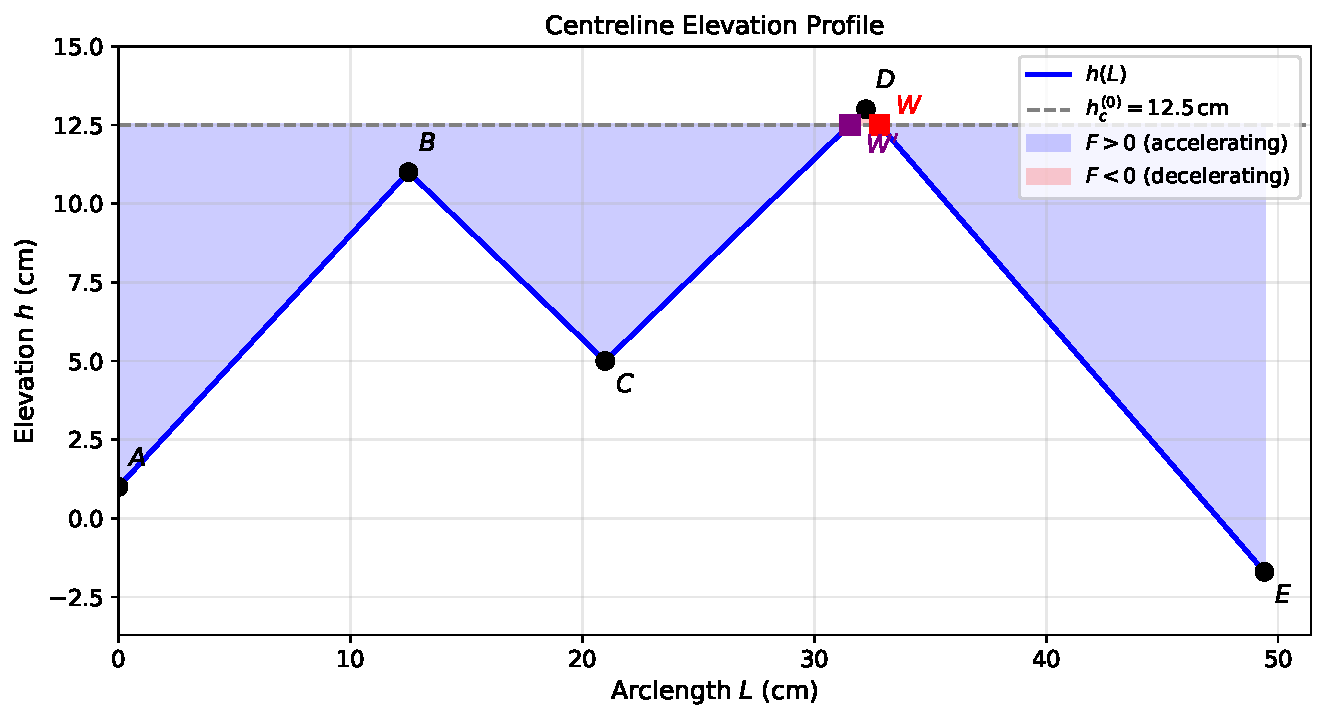
\includegraphics[width=0.85\textwidth]{figure2_centreline.pdf}
  \caption{Centreline elevation $h(L)$ versus arclength. The dashed line marks $h_c^{(0)} = 12.5$\,cm. Blue shading indicates positive driving force (front below waterline); red shading indicates negative driving force.}
  \label{fig:centreline}
\end{figure}

% --- FIGURE 4: Energy integral ---
\begin{figure}[H]
  \centering
  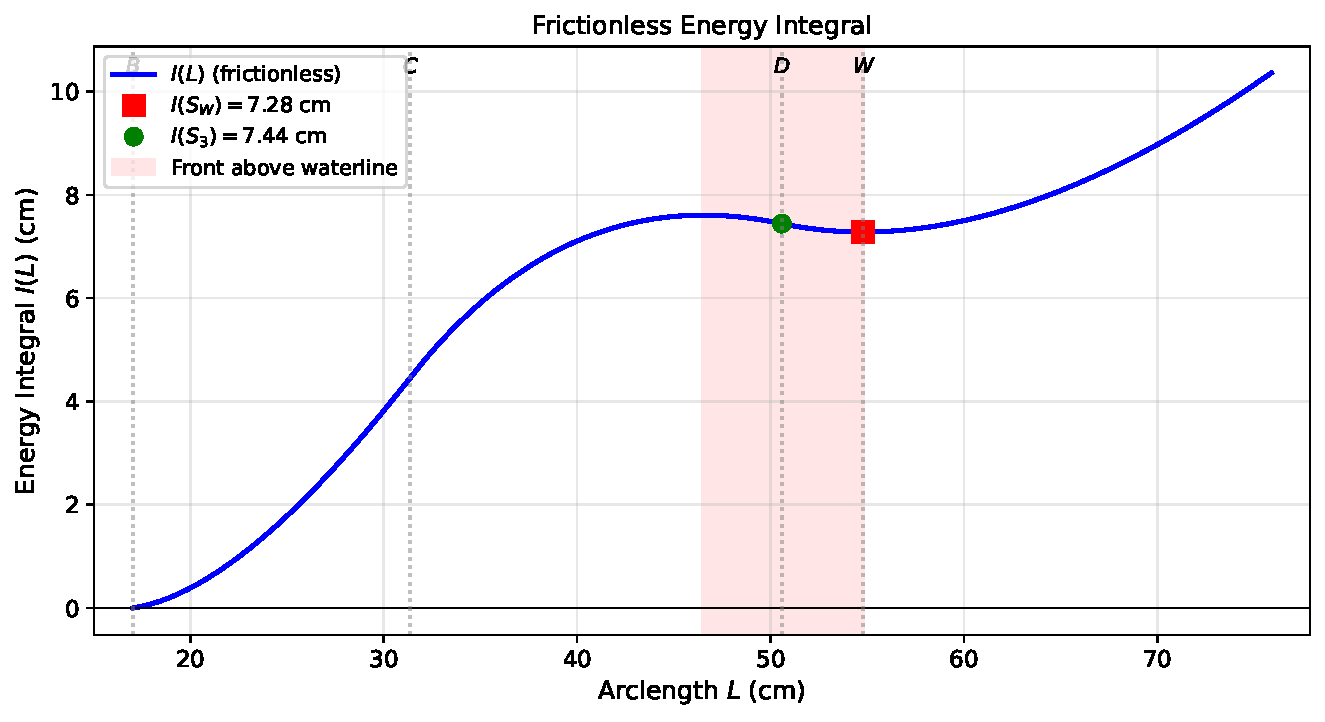
\includegraphics[width=0.85\textwidth]{figure4_energy_integral.pdf}
  \caption{Energy integral $I(L)$ versus arclength. The integral rises during the drop, continues rising while the front remains below the waterline on the climb, then decreases slightly between $W'$ and $W$. At $S_W$, $I(S_W) = 3.82\,\text{cm} > 0$: the frictionless priming criterion is satisfied.}
  \label{fig:energy-integral}
\end{figure}

% ══════════════════════════════════════════════════════════════════════════════
%  SECTION 5: DRAWDOWN EFFECTS
% ══════════════════════════════════════════════════════════════════════════════
\section{Adding Container Drawdown}
\label{sec:drawdown}

As water enters the pipe, the container level drops. This \emph{drawdown} reduces the driving force.

\subsection{Volume Conservation}

Water entering the pipe equals water leaving the container:
\begin{equation}
  A(L - S_1) = A_0[h_c^{(0)} - h_c(L)].
  \label{eq:volume-conservation}
\end{equation}

Solving for the container level:
\begin{equation}
  \boxed{h_c(L) = h_c^{(0)} - \frac{A}{A_0}(L - S_1)}
  \label{eq:drawdown}
\end{equation}

The level decreases linearly with slug position at rate $A/A_0$.

\subsection{Modified Energy Integral}

With variable container level, the energy integral becomes:
\begin{equation}
  I_{\text{dd}}(L) = \int_{S_1}^{L} \frac{h_c(r) - h(r)}{r}\,dr = I(L) - \frac{A}{A_0}\int_{S_1}^{L}\frac{r - S_1}{r}\,dr.
  \label{eq:I-dd}
\end{equation}

The drawdown penalty integral evaluates to:
\begin{equation}
  \int_{S_1}^{L}\frac{r - S_1}{r}\,dr = (L - S_1) - S_1\ln\frac{L}{S_1}.
  \label{eq:drawdown-penalty}
\end{equation}

\subsection{When Drawdown Matters}

The total drawdown by the outlet:
\begin{equation}
  \Delta h_c = \frac{A}{A_0}(L_{\max} - S_1).
  \label{eq:total-drawdown}
\end{equation}

For our experiment: $\Delta h_c = (5.77 \times 10^{-4}) \times 36.91 = 0.021$\,cm---negligible.

For a smaller container with $A_0 = 20\,\text{cm}^2$: $\Delta h_c \approx 0.36$\,cm, which is $24\%$ of the initial driving head at node $B$.

\begin{keyresult}
The area ratio $A/A_0$ controls drawdown importance:
\begin{itemize}[nosep]
  \item $A/A_0 \ll 0.01$: Drawdown negligible
  \item $A/A_0 \gtrsim 0.01$: Drawdown must be included
\end{itemize}
\end{keyresult}

% --- FIGURE 5: Drawdown ---
\begin{figure}[H]
  \centering
  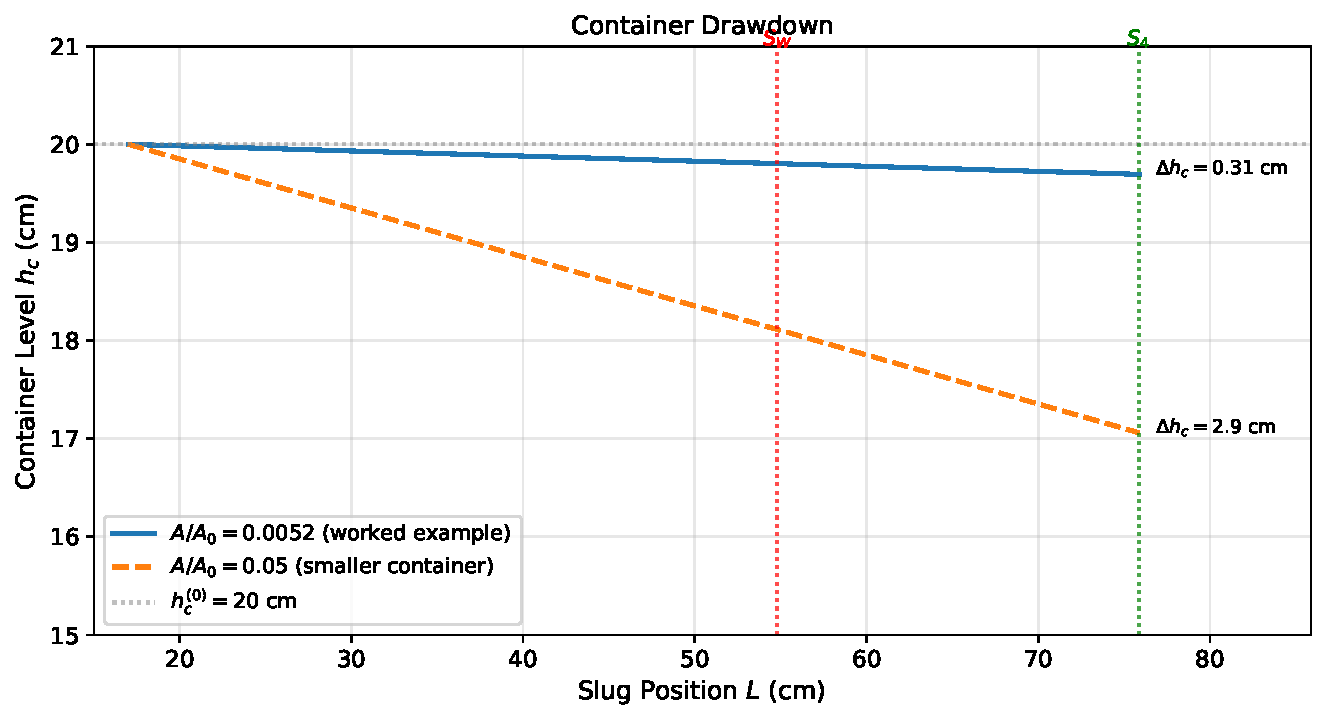
\includegraphics[width=0.85\textwidth]{figure5_drawdown.pdf}
  \caption{Container level $h_c(L)$ for two area ratios. The experimental case (solid) shows negligible drawdown; a smaller container (dashed) shows significant reduction in driving head.}
  \label{fig:drawdown}
\end{figure}

% ══════════════════════════════════════════════════════════════════════════════
%  SECTION 6: FRICTION EFFECTS
% ══════════════════════════════════════════════════════════════════════════════
\section{Adding Friction}
\label{sec:friction}

Viscous friction dissipates kinetic energy. We develop analytical results using constant friction, then discuss velocity-dependent friction.

\subsection{The Darcy-Weisbach Equation}

The head loss over pipe length $L$ is given by the Darcy-Weisbach equation \citep{brown2002history,darcy1857}:
\begin{equation}
  h_f = f\frac{L}{D}\frac{v^2}{2g},
  \label{eq:darcy-weisbach}
\end{equation}
where $f$ is the Darcy friction factor. This formulation, developed by Darcy and Weisbach in the 1840s and standardized by \citet{moody1944friction}, has become the universal method for pipe friction calculations.

Minor losses at bends and fittings add \citep{idelchik1994handbook}:
\begin{equation}
  h_{\text{minor}} = \sum K \frac{v^2}{2g},
  \label{eq:minor-losses}
\end{equation}
where $K$ values are tabulated for various fittings. Typical values range from $K \approx 0.3$ for gentle bends to $K \approx 1.5$ for sharp $90^\circ$ elbows.

\subsection{The Friction Factor}

The friction factor depends on Reynolds number $\text{Re} = vD/\nu$ and relative roughness $\varepsilon/D$. In the laminar regime ($\text{Re} < 2300$), the Hagen-Poiseuille solution gives \citep{hagen1839,poiseuille1840}:
\begin{equation}
  f = \frac{64}{\text{Re}} \quad \text{(laminar)}.
  \label{eq:f-laminar}
\end{equation}

In the turbulent regime, the Colebrook-White equation \citep{colebrook1939turbulent} provides:
\begin{equation}
  \frac{1}{\sqrt{f}} = -2\log\left(\frac{\varepsilon/D}{3.7} + \frac{2.51}{\text{Re}\sqrt{f}}\right) \quad \text{(turbulent)}.
  \label{eq:colebrook}
\end{equation}

For calculations spanning all regimes, we use the Churchill correlation \citep{churchill1977friction}:
\begin{equation}
  f = 8\left[\left(\frac{8}{\text{Re}}\right)^{12} + \frac{1}{(A_C + B_C)^{3/2}}\right]^{1/12},
  \label{eq:churchill}
\end{equation}
where $A_C$ and $B_C$ are functions of Re and $\varepsilon/D$ given in \cref{app:friction}. This correlation recovers the Hagen-Poiseuille result for laminar flow and matches Colebrook-White for turbulent flow.

\subsection{Constant-Friction Approximation}

Treating $f$ as constant enables analytical solution. With friction, the equation of motion becomes:
\begin{equation}
  v\frac{dv}{dL} + \left(\frac{f_0}{D} + \frac{\sum K}{L}\right)\frac{v^2}{2} = \frac{g[h_c^{(0)} - h(L)]}{L}.
  \label{eq:friction-eom}
\end{equation}

Substituting $u = v^2/2$ gives a linear first-order ODE:
\begin{equation}
  \frac{du}{dL} + \left(\frac{f_0}{D} + \frac{\sum K}{L}\right)u = \frac{g[h_c^{(0)} - h(L)]}{L}.
  \label{eq:u-ODE}
\end{equation}

The integrating factor is:
\begin{equation}
  \mu(L) = \left(\frac{L}{S_1}\right)^{\sum K}\exp\left(\frac{f_0(L - S_1)}{D}\right).
  \label{eq:integrating-factor}
\end{equation}

\begin{definition}[Friction-Corrected Energy Integral]
\begin{equation}
  \boxed{I_f(L) = \frac{1}{\mu(L)}\int_{S_1}^{L}\mu(r)\frac{h_c^{(0)} - h(r)}{r}\,dr}
  \label{eq:I-f}
\end{equation}
\end{definition}

\subsection{Physical Interpretation}

The effective weight for energy stored at position $r$ becomes:
\begin{equation}
  \frac{\mu(r)}{\mu(L)} \cdot \frac{1}{r} = \frac{1}{r}\left(\frac{r}{L}\right)^{\sum K}\exp\left(-\frac{f_0(L-r)}{D}\right).
  \label{eq:effective-weight}
\end{equation}

The exponential factor \emph{discounts} early contributions: energy stored early must travel farther and suffers more dissipation. This explains why $I_f(L) < I(L)$ always.

\subsection{Loss Estimation}

For our experiment, the measured peak velocity is $v \approx 36$\,cm/s, giving:
\begin{equation}
  \text{Re} = \frac{36 \times 0.5}{0.01} \approx 1800 \quad \text{(mostly laminar)}.
  \label{eq:Re-estimate}
\end{equation}

From \eqref{eq:f-laminar}, $f \approx 64/1800 \approx 0.036$.

Distributed friction loss over the full pipe:
\begin{equation}
  h_f \approx 0.036 \times \frac{49.4}{0.5} \times \frac{36^2}{2 \times 981} \approx 2.4\,\text{cm}.
  \label{eq:hf-estimate}
\end{equation}

Minor losses with fitted $\sum K \approx 14.4$:
\begin{equation}
  h_{\text{minor}} \approx 14.4 \times \frac{36^2}{2 \times 981} \approx 9.5\,\text{cm}.
  \label{eq:hminor-estimate}
\end{equation}

Minor losses dominate the energy budget for small-diameter siphons with tight bends.

% --- FIGURE 6: Friction factor ---
\begin{figure}[H]
  \centering
  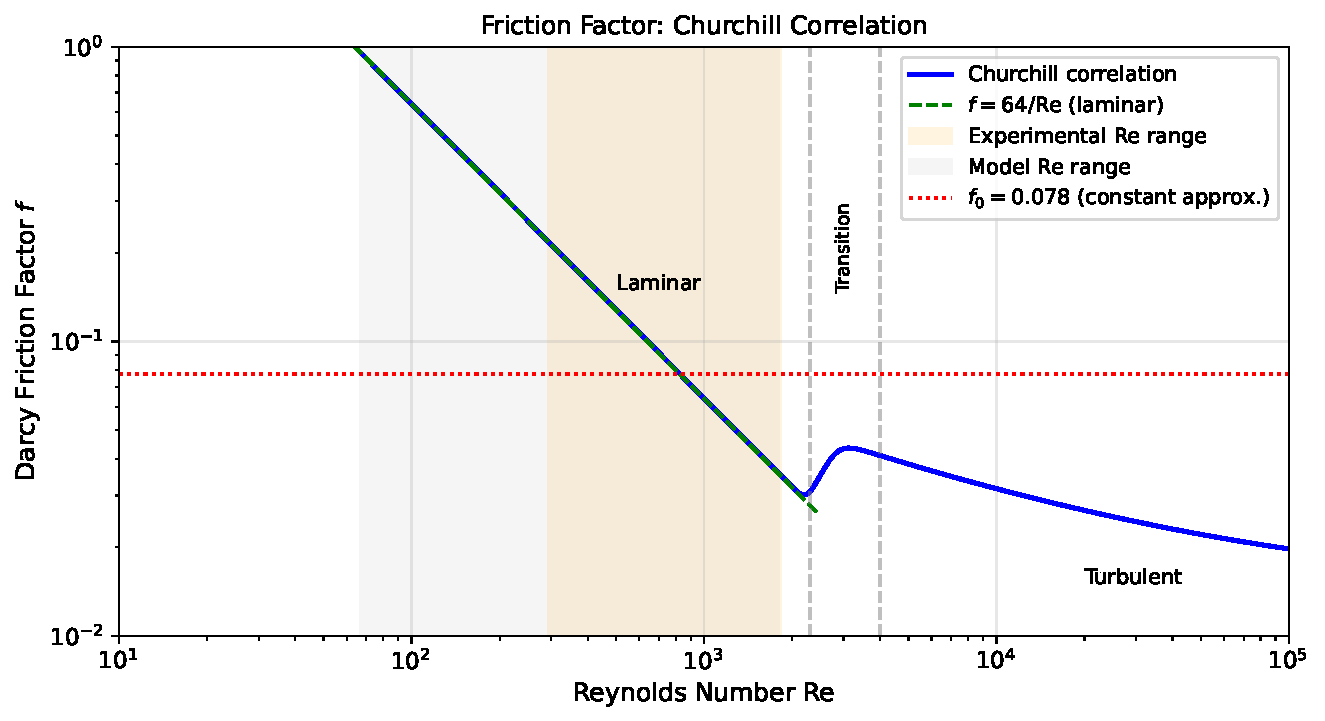
\includegraphics[width=0.85\textwidth]{figure6_friction.pdf}
  \caption{Friction factor $f$ versus Reynolds number from the Churchill correlation. The experimental range (shaded) is mostly in the laminar regime. The dashed line shows the constant approximation $f_0$.}
  \label{fig:friction}
\end{figure}

% ══════════════════════════════════════════════════════════════════════════════
%  SECTION 7: MODEL COMPARISON
% ══════════════════════════════════════════════════════════════════════════════
\section{Comparing the Three Models}
\label{sec:comparison}

The three energy integrals form a hierarchy:
\begin{equation}
  I(L) \geq I_{\text{dd}}(L) \geq I_f(L).
  \label{eq:hierarchy}
\end{equation}

\subsection{Values at Critical Point $S_W$}

\begin{center}
\renewcommand{\arraystretch}{1.3}
\begin{tabular}{lccc}
\toprule
Model & Integral at $S_W$ & Velocity at $W$ & Controlling Parameter \\
\midrule
Frictionless & $I = 3.82$\,cm & 86.5\,cm/s & Geometry \\
With drawdown & $I_{\text{dd}} = 3.81$\,cm & 86.4\,cm/s & $A/A_0$ \\
With friction & $I_f \approx 0.02$\,cm & 6.3\,cm/s & $\varepsilon/D$, $\sum K$ \\
\bottomrule
\end{tabular}
\end{center}

\subsection{Physical Insights}

\begin{itemize}[nosep,leftmargin=2em]
  \item \textbf{Frictionless integral:} The upper bound. Represents maximum kinetic energy from geometry alone.
  \item \textbf{Drawdown correction:} Negligible for large containers (our case).
  \item \textbf{Friction correction:} Dominates the energy budget. The 99\% reduction reflects severe discounting of early-stored energy by the $(L/S_1)^{\sum K}$ factor.
\end{itemize}

The constant-friction model is \emph{conservative}: it provides a lower bound that, while pessimistic, guarantees priming if $I_f(S_W) > 0$.

% --- FIGURE 7: Comparison ---
\begin{figure}[H]
  \centering
  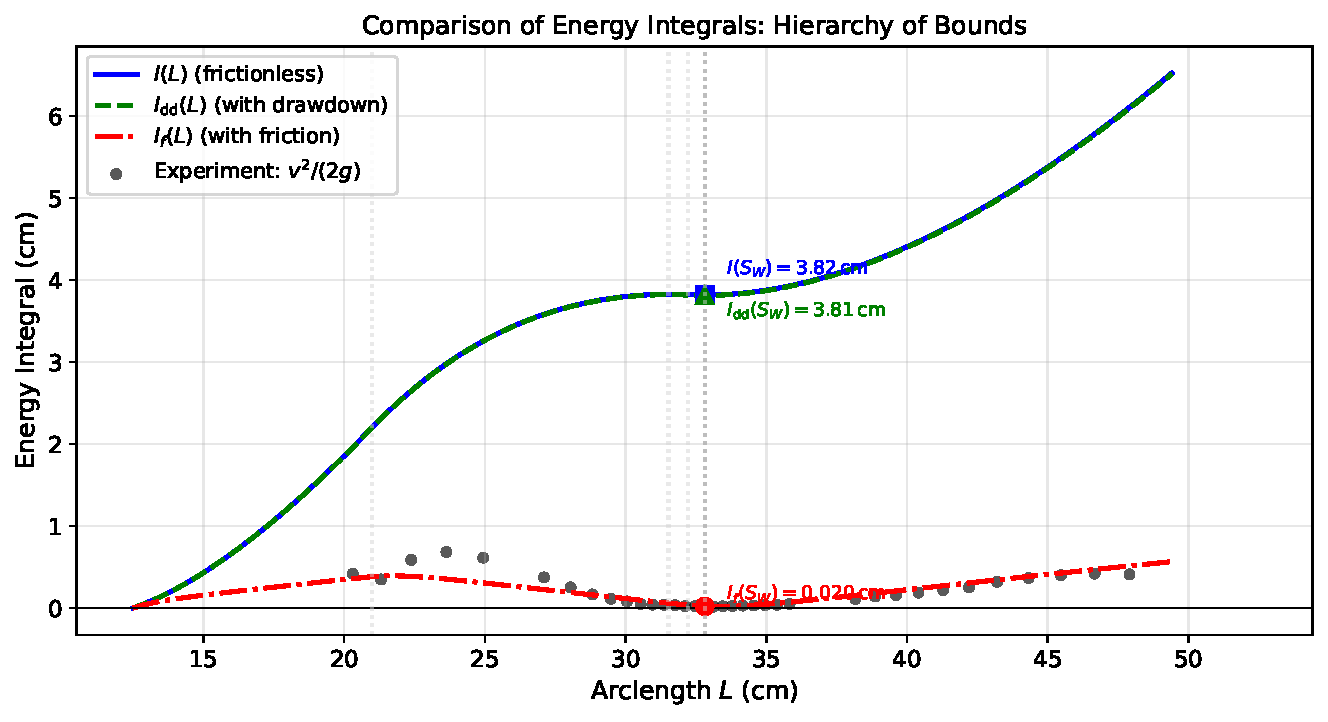
\includegraphics[width=0.85\textwidth]{figure7_comparison.pdf}
  \caption{Comparison of energy integrals versus arclength. The frictionless integral (solid) provides the upper bound; drawdown (dashed) reduces it slightly; friction (dash-dot) causes substantial reduction. Experimental kinetic head $v^2/(2g)$ shown as points.}
  \label{fig:comparison}
\end{figure}

% ══════════════════════════════════════════════════════════════════════════════
%  SECTION 8: NUMERICAL DYNAMICS
% ══════════════════════════════════════════════════════════════════════════════
\section{Full Numerical Dynamics}
\label{sec:dynamics}

The analytical integrals provide bounds, but accurate predictions require velocity-dependent friction.

\subsection{The Complete ODE System}

For filling ($L < L_{\max}$):
\begin{align}
  \frac{dL}{dt} &= v, \label{eq:ode-L} \\
  \frac{dv}{dt} &= \frac{g}{L}\left[h_c(L) - h(L)\right] - \left(\frac{f(\text{Re})}{D} + \frac{\sum K}{L}\right)\frac{v^2}{2}. \label{eq:ode-v}
\end{align}

At each step, $\text{Re} = vD/\nu$ is computed and $f$ evaluated from \eqref{eq:churchill}.

\subsection{Draining Phase}

Once the pipe fills completely ($L = L_{\max}$), the slug length is constant:
\begin{align}
  \frac{dh_c}{dt} &= -\frac{A}{A_0}v, \label{eq:drain-hc} \\
  \frac{dv}{dt} &= \frac{g[h_c - h_4]}{L_{\max}} - \left(\frac{f}{D} + \frac{\sum K}{L_{\max}}\right)\frac{v^2}{2}. \label{eq:drain-v}
\end{align}

For quasi-steady draining (large containers), setting $dv/dt = 0$:
\begin{equation}
  v_{\text{qs}} = \sqrt{\frac{2g(h_c - h_4)}{fL_{\max}/D + \sum K}}.
  \label{eq:quasi-steady}
\end{equation}

\subsection{Draining Time Estimate}

Integrating the quasi-steady approximation:
\begin{equation}
  t_{\text{drain}} = \frac{2A_0}{A}\sqrt{\frac{fL_{\max}/D + \sum K}{2g}}\sqrt{h_c^{(0)} - h_4}.
  \label{eq:drain-time}
\end{equation}

For our experiment: $t_{\text{drain}} \approx 23$\,min---much longer than filling due to friction-limited steady-state velocity.

% ══════════════════════════════════════════════════════════════════════════════
%  SECTION 9: EXPERIMENTS
% ══════════════════════════════════════════════════════════════════════════════
\section{Comparison with Experiment}
\label{sec:experiments}

\subsection{Setup}

The experimental siphon was constructed from 5\,mm inner diameter flexible tubing bent around a rigid frame to maintain the five-node geometry. The container was a rectangular tank with $A_0 = 340\,\text{cm}^2$ cross-section.

\subsection{Video Tracking}

High-speed video (120 fps) captured the filling process. The water front position was extracted frame-by-frame using edge detection. Velocity was computed from position differences using a Savitzky-Golay filter to reduce noise.

\subsection{Results}

\Cref{fig:velocity,fig:time} compare model predictions with experimental data. Key observations:
\begin{itemize}[nosep,leftmargin=2em]
  \item The frictionless model overestimates velocity by a factor of $\sim 2$.
  \item The constant-friction model underestimates velocity (conservative bound).
  \item The full numerical model captures the essential dynamics.
  \item Peak measured velocity: $\sim 36$\,cm/s at low point $C$.
  \item Filling time to outlet: $\sim 2$\,s.
\end{itemize}

The effective minor loss coefficient $\sum K \approx 14.4$ was obtained by fitting the numerical model to the measured $v(L)$ curve. This value is higher than handbook estimates for smooth bends, likely due to:
\begin{enumerate}[nosep,leftmargin=2em]
  \item Tight bend radii in our geometry
  \item Entrance and exit effects not separately modeled
  \item Developing flow in short segments
\end{enumerate}

% --- FIGURE 8: Velocity ---
\begin{figure}[H]
  \centering
  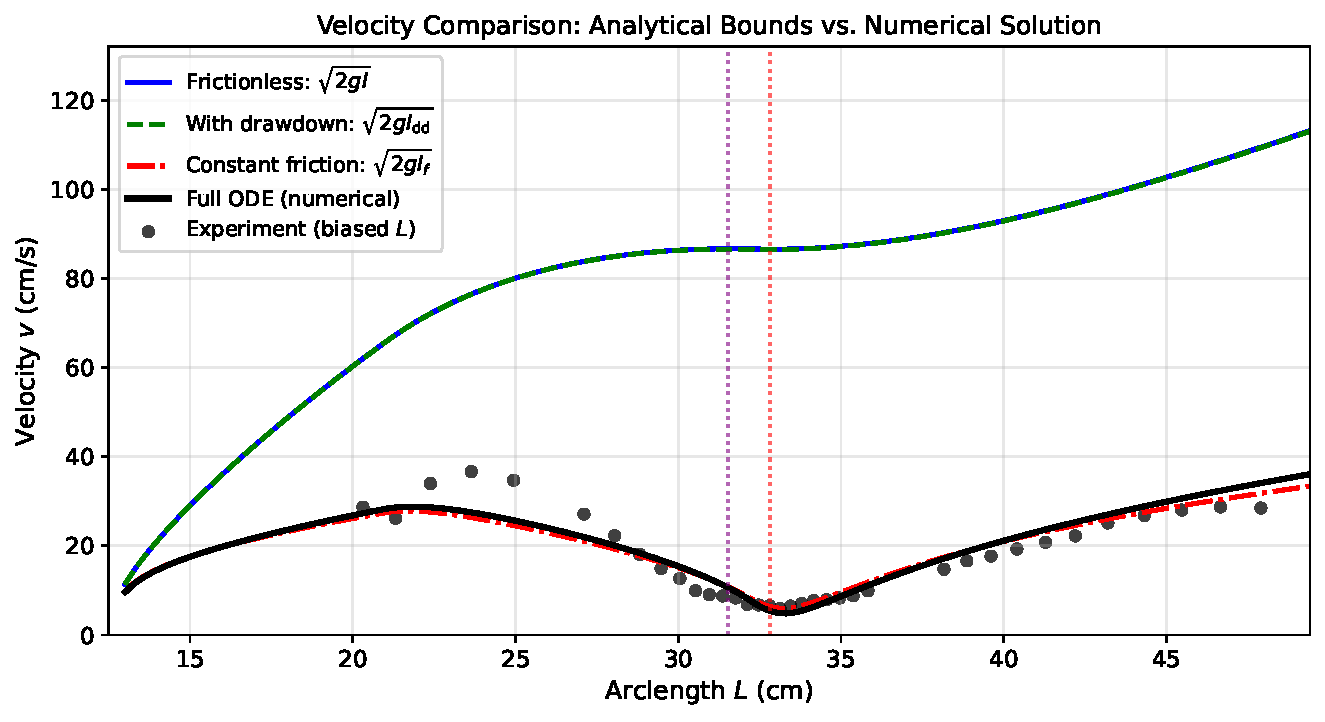
\includegraphics[width=0.85\textwidth]{figure8_velocity.pdf}
  \caption{Velocity $v(L)$ during filling. Model curves: frictionless (upper bound), constant friction (lower bound), full ODE (best estimate). Experimental points track the full model reasonably well.}
  \label{fig:velocity}
\end{figure}

% --- FIGURE 9: Time evolution ---
\begin{figure}[H]
  \centering
  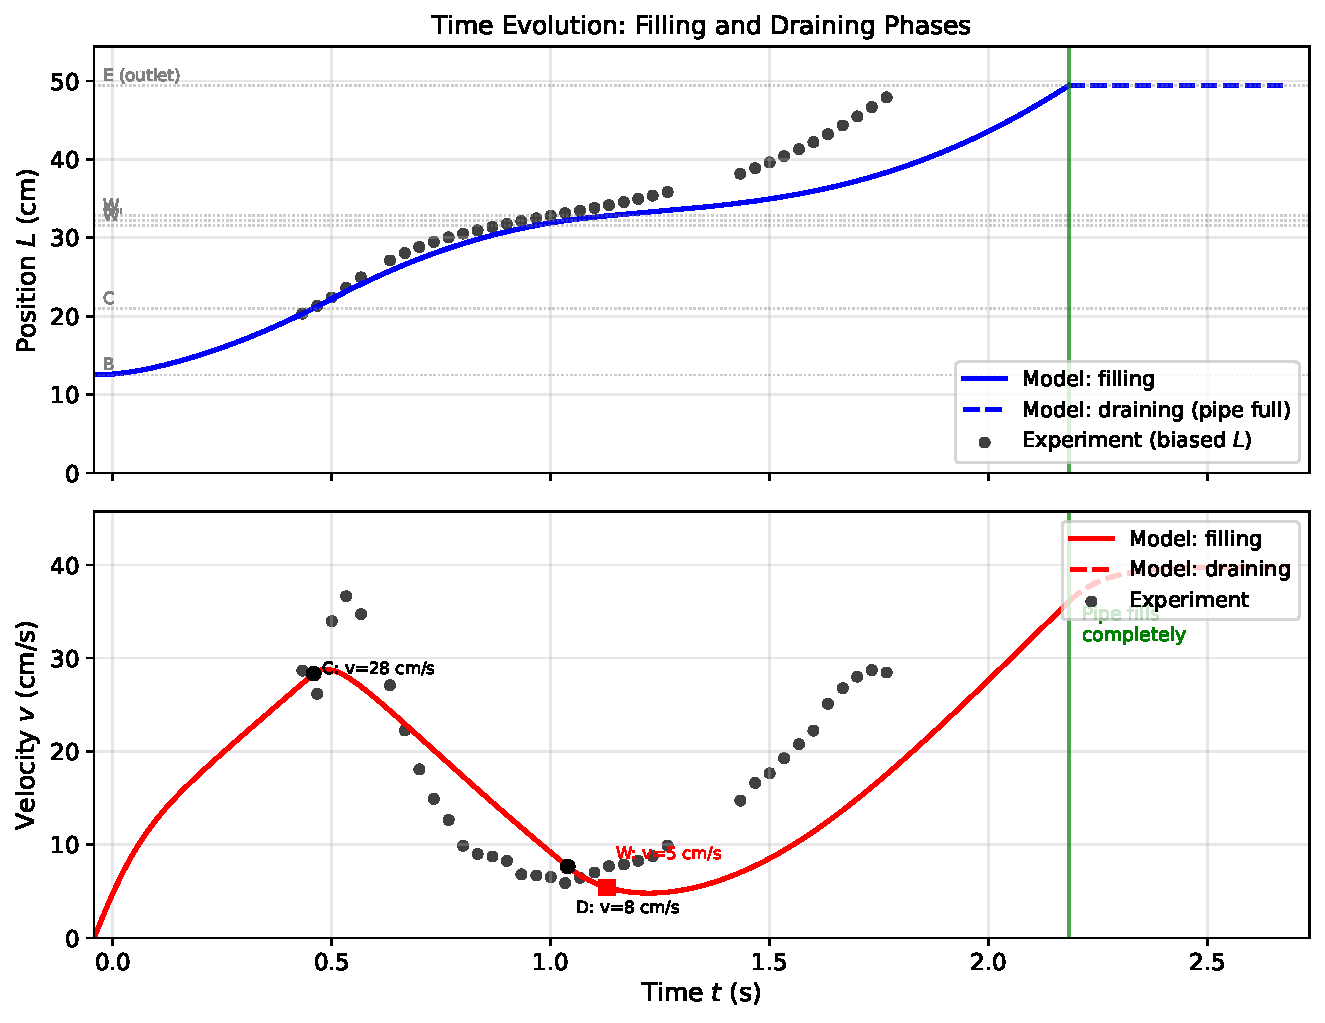
\includegraphics[width=0.85\textwidth]{figure9_time.pdf}
  \caption{Position $L(t)$ and velocity $v(t)$ versus time. Model curves are time-shifted to align with experimental start. Key positions (C, D, W, outlet) are marked.}
  \label{fig:time}
\end{figure}

% ══════════════════════════════════════════════════════════════════════════════
%  SECTION 10: VALIDITY LIMITS
% ══════════════════════════════════════════════════════════════════════════════
\section{Validity Limits}
\label{sec:validity}

Every model has a domain of validity. We quantify when each assumption fails using dimensionless parameters.

\subsection{Cavitation}

At the crest, pressure is minimum. Cavitation occurs when pressure drops below the vapor pressure $p_v \approx 2.3$\,kPa \citep{brennen1995cavitation}:
\begin{equation}
  p_D = p_{\text{atm}} - \rho g(h_3 - h_c) - \frac{\rho v^2}{2} - \rho g h_f > p_v.
  \label{eq:cavitation}
\end{equation}

The maximum siphon height is approximately 10\,m for water at sea level. For our geometry with $h_3 - h_c = 0.5$\,cm, cavitation is not a concern.

\subsection{Capillarity}

Surface tension effects become important at small diameters. Two dimensionless numbers characterize the regime \citep{degennes2004capillarity}:

\begin{definition}[Bond Number]
\begin{equation}
  \text{Bo} = \frac{\rho g D^2}{\gamma}
  \label{eq:bond}
\end{equation}
compares gravitational to surface tension forces. Gravity dominates when $\text{Bo} \gg 1$.
\end{definition}

\begin{definition}[Capillary Number]
\begin{equation}
  \text{Ca} = \frac{\mu v}{\gamma}
  \label{eq:capillary}
\end{equation}
compares viscous to surface tension forces. Dynamic meniscus effects are negligible when $\text{Ca} \ll 1$.
\end{definition}

For our experiment: $\text{Bo} \approx 3.4$ and $\text{Ca} \approx 0.005$. With $\text{Bo}$ only marginally above 1, capillary effects may contribute at the 10-20\% level.

\subsection{Entrance Effects}

The laminar entrance length scales as \citep{white2011fluid}:
\begin{equation}
  \frac{L_e}{D} \approx 0.05\,\text{Re}.
  \label{eq:entrance-length}
\end{equation}

At $\text{Re} \approx 1800$, this gives $L_e \approx 45$\,cm---comparable to segment lengths. The quasi-steady friction assumption is therefore marginal.

\subsection{Secondary Flows}

Flow through bends generates Dean vortices, characterized by the Dean number \citep{dean1927motion}:
\begin{equation}
  \text{De} = \text{Re}\sqrt{\frac{D}{2R}},
  \label{eq:dean}
\end{equation}
where $R$ is the bend radius. Secondary flows become significant when $\text{De} > 100$ \citep{berger1983flow}.

For our tight bends with $R \approx 2D$: $\text{De} \approx 900$, indicating strong secondary flows that justify treating bend losses as lumped $K$ values rather than distributed friction.

\subsection{Unsteady Friction}

The Womersley number characterizes oscillatory effects \citep{womersley1955method}:
\begin{equation}
  \text{Wo} = D\sqrt{\frac{\omega}{\nu}},
  \label{eq:womersley}
\end{equation}
where $\omega \sim 1/T$ is the frequency of velocity variation. For $T \sim 0.5$\,s: $\text{Wo} \approx 5$. Unsteady effects are modest but not negligible.

\subsection{Regime Diagrams}

\Cref{fig:validity} summarizes validity limits in three parameter spaces.

% --- FIGURE 10: Validity ---
\begin{figure}[H]
  \centering
  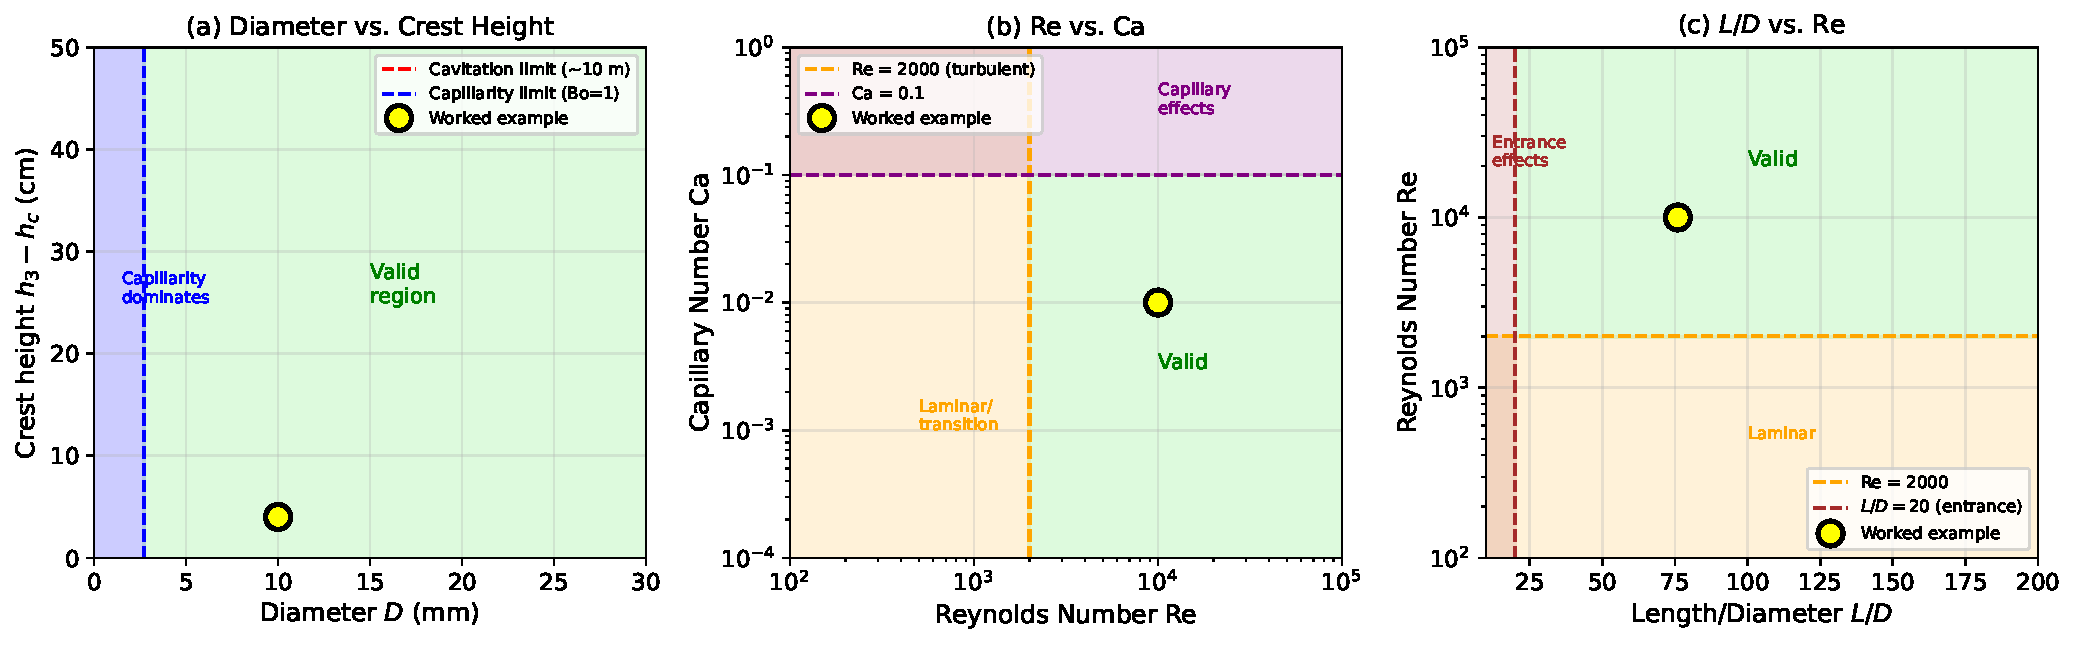
\includegraphics[width=0.95\textwidth]{figure10_validity.pdf}
  \caption{Validity regime diagrams. (a) Diameter vs. crest height: cavitation limits tall crests; capillarity limits small diameters. (b) Re vs. Ca: shows laminar/turbulent boundary and capillary regime. (c) $L/D$ vs. Re: entrance effects become important at low $L/D$ or high Re. The experimental point (marked) lies near the capillary and entrance-effect boundaries.}
  \label{fig:validity}
\end{figure}

% ══════════════════════════════════════════════════════════════════════════════
%  SECTION 11: CONCLUSION
% ══════════════════════════════════════════════════════════════════════════════
\section{Conclusion}
\label{sec:conclusion}

We developed a theoretical framework for self-starting siphons through systematic derivation from the Navier-Stokes equations and layered incorporation of physical effects.

\subsection{Key Results}

\begin{enumerate}[nosep,leftmargin=2em]
  \item \textbf{Geometry is fundamental.} The frictionless energy integral $I(L)$ determines whether priming is geometrically possible. The criterion $I(S_W) > 0$ provides a closed-form screening tool.

  \item \textbf{Friction dominates losses.} For small-diameter siphons with tight bends, minor losses ($\sum K$) typically exceed distributed friction ($fL/D$). Reducing bend losses is more effective than smoothing pipe walls.

  \item \textbf{Drawdown matters for small containers.} When $A/A_0 > 0.01$, container level drop significantly reduces driving head.

  \item \textbf{Analytical bounds bracket reality.} The hierarchy $I \geq I_{\text{dd}} \geq I_f$ provides physical insight that numerical simulation alone cannot offer.

  \item \textbf{Validity limits are quantifiable.} Dimensionless parameters (Bo, Ca, De, Wo) identify when assumptions fail. Our experiment lies near the capillary and entrance-effect boundaries.
\end{enumerate}

\subsection{Design Guidelines}

For reliable self-starting:
\begin{itemize}[nosep,leftmargin=2em]
  \item Maximize the early drop ($B \to C$) to build momentum when the slug is short
  \item Minimize crest height ($h_3 - h_c^{(0)}$) while maintaining positive margin
  \item Use gentle bends with large radii to reduce $K$ values
  \item Prefer larger diameters to reduce friction and capillary effects
  \item Ensure adequate container size if drawdown matters
\end{itemize}

\subsection{Future Work}

Extensions could address:
\begin{itemize}[nosep,leftmargin=2em]
  \item Systematic optimization of geometry for minimum filling time
  \item Inclusion of capillary effects for sub-5\,mm diameters
  \item Unsteady friction corrections for rapid transients
  \item Two-phase flow effects during initial priming
\end{itemize}

% ══════════════════════════════════════════════════════════════════════════════
%  APPENDIX: FRICTION CORRELATIONS
% ══════════════════════════════════════════════════════════════════════════════
\appendix
\section{Friction Correlations}
\label{app:friction}

\subsection{The Churchill Correlation}

The Churchill correlation \citep{churchill1977friction} provides a single formula valid across all flow regimes:
\begin{equation}
  f = 8\left[\left(\frac{8}{\text{Re}}\right)^{12} + \frac{1}{(A_C + B_C)^{3/2}}\right]^{1/12},
  \label{eq:churchill-full}
\end{equation}
where
\begin{align}
  A_C &= \left[2.457\ln\left(\frac{1}{(7/\text{Re})^{0.9} + 0.27(\varepsilon/D)}\right)\right]^{16}, \\
  B_C &= \left(\frac{37530}{\text{Re}}\right)^{16}.
\end{align}

\subsection{Limiting Behavior}

\paragraph{Laminar limit ($\text{Re} \to 0$):}
The first term dominates: $f \to 64/\text{Re}$, recovering Hagen-Poiseuille.

\paragraph{Turbulent limit ($\text{Re} \to \infty$):}
The second term dominates, recovering Colebrook-White.

\paragraph{Transition:}
Smooth interpolation provides continuous, differentiable $f(\text{Re})$.

% --- FIGURE A1: Friction comparison ---
\begin{figure}[H]
  \centering
  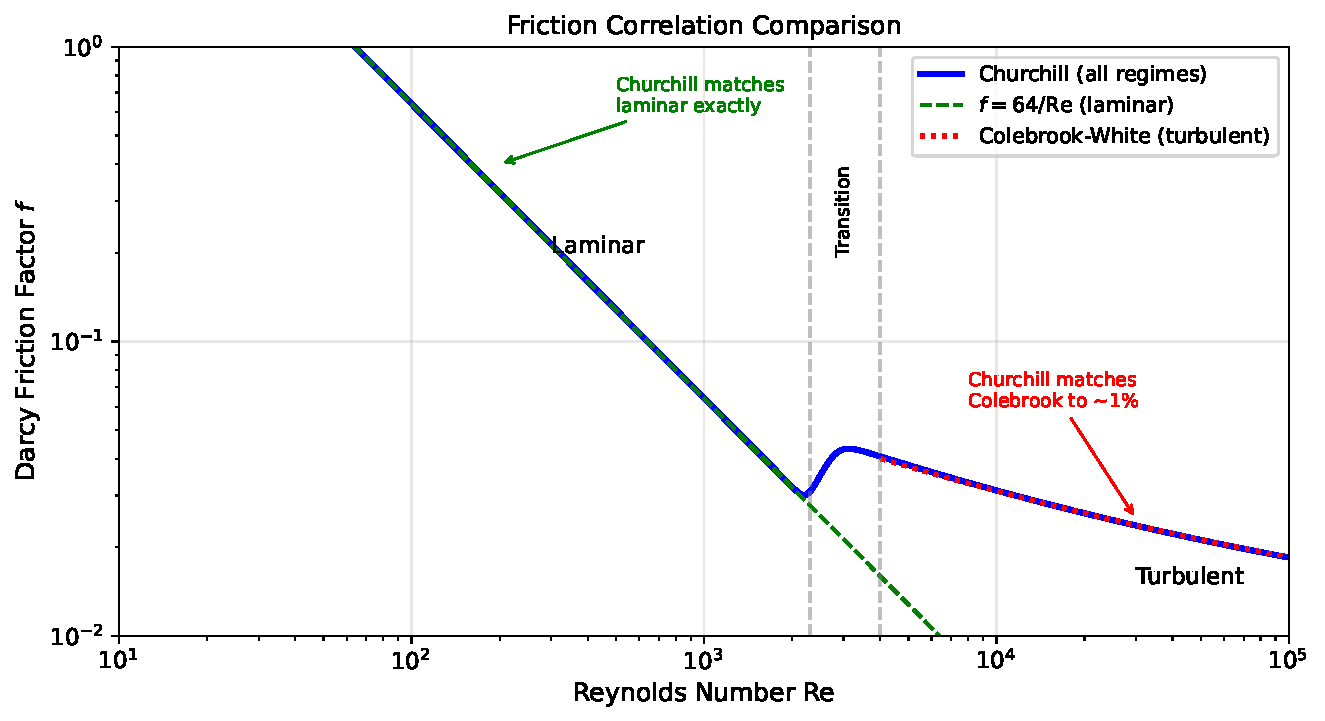
\includegraphics[width=0.85\textwidth]{figureA1_friction_comparison.pdf}
  \caption{Comparison of friction correlations. The Churchill correlation (solid) matches the laminar law exactly and Colebrook-White (dotted, turbulent only) to within 1\%.}
  \label{fig:friction-comparison}
\end{figure}

% ══════════════════════════════════════════════════════════════════════════════
%  BIBLIOGRAPHY
% ══════════════════════════════════════════════════════════════════════════════
\bibliographystyle{apalike}
\begin{thebibliography}{99}

\bibitem[Batchelor(1967)]{batchelor1967introduction}
Batchelor, G.~K. (1967).
\newblock {\em An Introduction to Fluid Dynamics}.
\newblock Cambridge University Press.

\bibitem[Berger et~al.(1983)]{berger1983flow}
Berger, S.~A., Talbot, L., \& Yao, L.-S. (1983).
\newblock Flow in curved pipes.
\newblock {\em Annual Review of Fluid Mechanics}, 15:461--512.

\bibitem[Boatwright et~al.(2015)]{boatwright2015siphon}
Boatwright, A., Hughes, S., \& Barry, J. (2015).
\newblock The height limit of a siphon.
\newblock {\em Scientific Reports}, 5:16790.

\bibitem[Brennen(1995)]{brennen1995cavitation}
Brennen, C.~E. (1995).
\newblock {\em Cavitation and Bubble Dynamics}.
\newblock Oxford University Press.

\bibitem[Brown(2002)]{brown2002history}
Brown, G.~O. (2002).
\newblock The history of the {D}arcy-{W}eisbach equation for pipe flow resistance.
\newblock In {\em Environmental and Water Resources History}, pages 34--43. ASCE.

\bibitem[Churchill(1977)]{churchill1977friction}
Churchill, S.~W. (1977).
\newblock Friction-factor equation spans all fluid-flow regimes.
\newblock {\em Chemical Engineering}, 84(24):91--92.

\bibitem[Colebrook(1939)]{colebrook1939turbulent}
Colebrook, C.~F. (1939).
\newblock Turbulent flow in pipes, with particular reference to the transition region between the smooth and rough pipe laws.
\newblock {\em Journal of the Institution of Civil Engineers}, 11(4):133--156.

\bibitem[Darcy(1857)]{darcy1857}
Darcy, H. (1857).
\newblock {\em Recherches exp\'{e}rimentales relatives au mouvement de l'eau dans les tuyaux}.
\newblock Mallet-Bachelier, Paris.

\bibitem[Dean(1927)]{dean1927motion}
Dean, W.~R. (1927).
\newblock Note on the motion of fluid in a curved pipe.
\newblock {\em The London, Edinburgh, and Dublin Philosophical Magazine and Journal of Science}, 4(20):208--223.

\bibitem[de~Gennes et~al.(2004)]{degennes2004capillarity}
de~Gennes, P.-G., Brochard-Wyart, F., \& Qu\'{e}r\'{e}, D. (2004).
\newblock {\em Capillarity and Wetting Phenomena: Drops, Bubbles, Pearls, Waves}.
\newblock Springer.

\bibitem[Fox et~al.(2011)]{fox2011introduction}
Fox, R.~W., McDonald, A.~T., \& Pritchard, P.~J. (2011).
\newblock {\em Introduction to Fluid Mechanics}.
\newblock John Wiley \& Sons, 8th edition.

\bibitem[Hagen(1839)]{hagen1839}
Hagen, G. (1839).
\newblock {\"U}ber die {B}ewegung des {W}assers in engen cylindrischen {R}{\"o}hren.
\newblock {\em Annalen der Physik}, 122(3):423--442.

\bibitem[Idelchik(1994)]{idelchik1994handbook}
Idelchik, I.~E. (1994).
\newblock {\em Handbook of Hydraulic Resistance}.
\newblock CRC Press, 3rd edition.

\bibitem[McDonald(2024)]{mcdonald2024siphon}
McDonald, K.~T. (2024).
\newblock Forces on a siphon.
\newblock Princeton University Technical Report.

\bibitem[Moody(1944)]{moody1944friction}
Moody, L.~F. (1944).
\newblock Friction factors for pipe flow.
\newblock {\em Transactions of the ASME}, 66(8):671--684.

\bibitem[Plastino \& Muzzio(1992)]{plastino1992}
Plastino, A.~R. \& Muzzio, J.~C. (1992).
\newblock On the use and abuse of {N}ewton's second law for variable mass problems.
\newblock {\em Celestial Mechanics and Dynamical Astronomy}, 53:227--232.

\bibitem[Poiseuille(1840)]{poiseuille1840}
Poiseuille, J.~L. (1840).
\newblock Recherches exp\'{e}rimentales sur le mouvement des liquides dans les tubes de tr\`{e}s-petits diam\`{e}tres.
\newblock {\em Comptes Rendus}, 11:961--967.

\bibitem[Potter \& Barnes(1971)]{potter2012siphon}
Potter, A. \& Barnes, F.~H. (1971).
\newblock The siphon.
\newblock {\em Physics Education}, 6(5):362--366.

\bibitem[White(2011)]{white2011fluid}
White, F.~M. (2011).
\newblock {\em Fluid Mechanics}.
\newblock McGraw-Hill, 7th edition.

\bibitem[Womersley(1955)]{womersley1955method}
Womersley, J.~R. (1955).
\newblock Method for the calculation of velocity, rate of flow and viscous drag in arteries when the pressure gradient is known.
\newblock {\em The Journal of Physiology}, 127(3):553--563.

\end{thebibliography}

\end{document}
